% !TEX root = thesis.tex

%%
%%
%% Results chapter
%%
%%

This chapter describes the results of several experiments, each run with a variation of the same setup.
In each case, we compare the results of 1,000 simulations using several accuracy measures.
Each section describes a set of experiments, which, together, examine the effect of changes to a single variable on the performance of the \gls{dkd}.

%%%%%%%%%%%%%%%%%%%%%%%%%%%%%%%%%%%%%%%%%%%%%%%%%%%%%%%%%%%%%%%%%%%%%%%%%%%%%%
%%
%% Section: Experimental setup
%%
%%%%%%%%%%%%%%%%%%%%%%%%%%%%%%%%%%%%%%%%%%%%%%%%%%%%%%%%%%%%%%%%%%%%%%%%%%%%%%
\section{Experimental setup}
\label{sec:results:setup}

Each experiment was run on one of \textit{c4.2xlarge} or \textit{c4.4xlarge} instance in Amazon AWS \citep{aws:instancetypes}.
These virtual machines have 8 and 16 virtual CPUs respectively.
This allowed the monte carlo simulations to be sped up by running in 7 or 15 parallel threads using the \texttt{parallel} package in \texttt{R} \citep{r:parallel}.
Randomization in parallel requires the random number stream to be split into separate sub-streams for each thread. 
This was done using the L'Ecuyer-CMRG method \citep{lecuyer2002random}.

Each experiment was run according to a set of parameters that comprised the particular setup.
The parameters (\cref{tab:experimental_parameters}) that define the study area remained fixed throughout the study.
In particular, we set \texttt{x1.min} to -4, \texttt{x1.max} to 4, \texttt{x2.min} to -4, \texttt{x2.max} to 4, and \texttt{buffer} to 0.5.
This gave us a study area with dimensions $8 \times 8$, with incidents concentrated in an area of $7 \times 7$.
For evaluating the \gls{dkd} we used a grid size of 0.5.

A table similar to \cref{tab:params:template}, describing the parameter ranges used in the related experiments appears at the beginning of each section below.
This table summarizes the values from \cref{tab:experimental_parameters} that are used to run the experiments in that section.
The first row in the table contains the \textit{population size} or \textit{sizes} used in the experiment.
The second row contains the \textit{population \gls{spread}}, which controls how quickly the population density drops from the peak.
We use the standard deviation \ensuremath\sigma of an independent, bivariate normal distribution with equal variances for this.
The third row in the the table contains the \textit{population center}, which is the point $\xvec$ of the peak of the population distribution.
For a uniform population distribution, the word ``uniform'' appears.
The next row in the table is the \gls{factor}.
This value is used to increase the expected number of cases for each simulation in the experiment.
It is the same \gls{mu} found in \cref{ch:method}.
The fifth row contains the \textit{incident \gls{spread}}, which controls how quickly the incidence risk drops from the peak.
We use the standard deviation \ensuremath\sigma of an independent, bivariate normal distribution with equal variances for this.
The sixth and last row in the the table contains the \textit{incident center}, which is the point $\xvec$ of the peak of the incident risk function.

%%%%%%%%%%%%%%%%%%%%%%%%%%%%%%%%%%%%%%%%%%%%%%%%%
% Parameter table - template
%%%%%%%%%%%%%%%%%%%%%%%%%%%%%%%%%%%%%%%%%%%%%%%%%
\begin{table}[htbp]
    \centering
    \begin{tabular}{ll}
        \hline
        Parameter & Value \\
        \hline
        Population size & 10,000 \\
        Population \glsentryname{spread} & 1.0 \\
        Population center & (0,0) \\
        \Glsentryname{factor} & 100, 200 \\
        Incident \glsentryname{spread} & 1.0 \\
        Incident center & (0,0) \\
        \hline
    \end{tabular}
    \caption{Experimental parameters template and example values}
    \label{tab:params:template}
\end{table}

In \cref{sec:results:unif_100_1.0_1h} we take a deep look at a single experiment.
The rest of this chapter examines the effect of different variables on the \gls{dkd} accuracy, on the selected bandwidths, and on other statistical properties of the \gls{dkd}.
\Cref{sec:results:number_of_incidents} describes the relationship between the accuracy of the \gls{dkd} and the magnitude of the risk function for a fixed population.
In \cref{sec:results:spread} we look at how the spread of the risk function affects accuracy.
We then made ran several sets of experiments while changing one parameter at a time.
\Cref{sec:results:unifNpop_1h} compares the results obtained by varying the size of the population.

%%%%%%%%%%%%%%%%%%%%%%%%%%%%%%%%%%%%%%%%%%%%%%%%%%%%%%%%%%%%%%%%%%%%%%%%%%%%%%
%%
%% Section: Results of single-peak risk on uniform population
%%
%%%%%%%%%%%%%%%%%%%%%%%%%%%%%%%%%%%%%%%%%%%%%%%%%%%%%%%%%%%%%%%%%%%%%%%%%%%%%%
\section[Results of single-peak risk on uniform population]
    {Results of a single experiment with risk function having single peak with with \glsentryname{spread} 1.0 and \glsentryname{factor} of 100 on a fixed, uniform population of 10,000}
\label{sec:results:unif_100_1.0_1h}
\graphicspath{{./results/unif_100_1.0_1h/}}
\makeatletter
\def\input@path{{./results/unif_100_1.0_1h/}}
\makeatother

In this section, we look at how well the \gls{dkd} performs when there is a single, central cause of disease incidents.
The strength of this source to generate incidents degrades with the distance from it.
We simulate this phenomenon with a risk function having a single peak with with \glsentryname{spread} 1.0 and \glsentryname{factor} of 100 on a fixed, uniform population of 10,000.
These parameters are summarized in \cref{tab:params:unif_100_1.0_1h}.
\Cref{fig:cases_scatter:unif_100_1.0_1h} shows a realization, generated from the model.
The distribution of the population in \subref{fig:cases_scatter:unif_100_1.0_1h:popdist},
the population points that were generated in \subref{fig:cases_scatter:unif_100_1.0_1h:poppts},
and the incidents on top of the population in \subref{fig:cases_scatter:unif_100_1.0_1h:incidentspts}.

%%%%%%%%%%%%%%%%%%%%%%%%%%%%%%%%%%%%%%%%%%%%%%%%%
% Parameter table - unif_100_1.0_1h
%%%%%%%%%%%%%%%%%%%%%%%%%%%%%%%%%%%%%%%%%%%%%%%%%
\begin{table}[htbp]
    \centering
    \begin{tabular}{ll}
        \hline
        Parameter & Value \\
        \hline
        Population size & 10,000 \\
        Population \glsentryname{spread} & uniform \\
        Population center & uniform \\
        \Glsentryname{factor} & 100 \\
        Incident \glsentryname{spread} & 1.0 \\
        Incident center & (0,0) \\
        \hline
    \end{tabular}
    \caption[Parameters of single-peak risk of 100 on uniform population]
        {Parameters used in a single experiment with a single-peak risk of \glsentryname{factor} 100 with \glsentryname{spread} of 1.0 on uniform population of 10,000.}
    \label{tab:params:unif_100_1.0_1h}
\end{table}


%%%%%%%%%%%%%%%%%%%%%%%%%%%%%%%%%%%%%%%%%%%%%%%%%
% Example cases scatter - unif_100_1.0_1h
%%%%%%%%%%%%%%%%%%%%%%%%%%%%%%%%%%%%%%%%%%%%%%%%%
\begin{figure}[htbp]
    \centering
    \begin{subfigure}[t]{0.32\textwidth}
        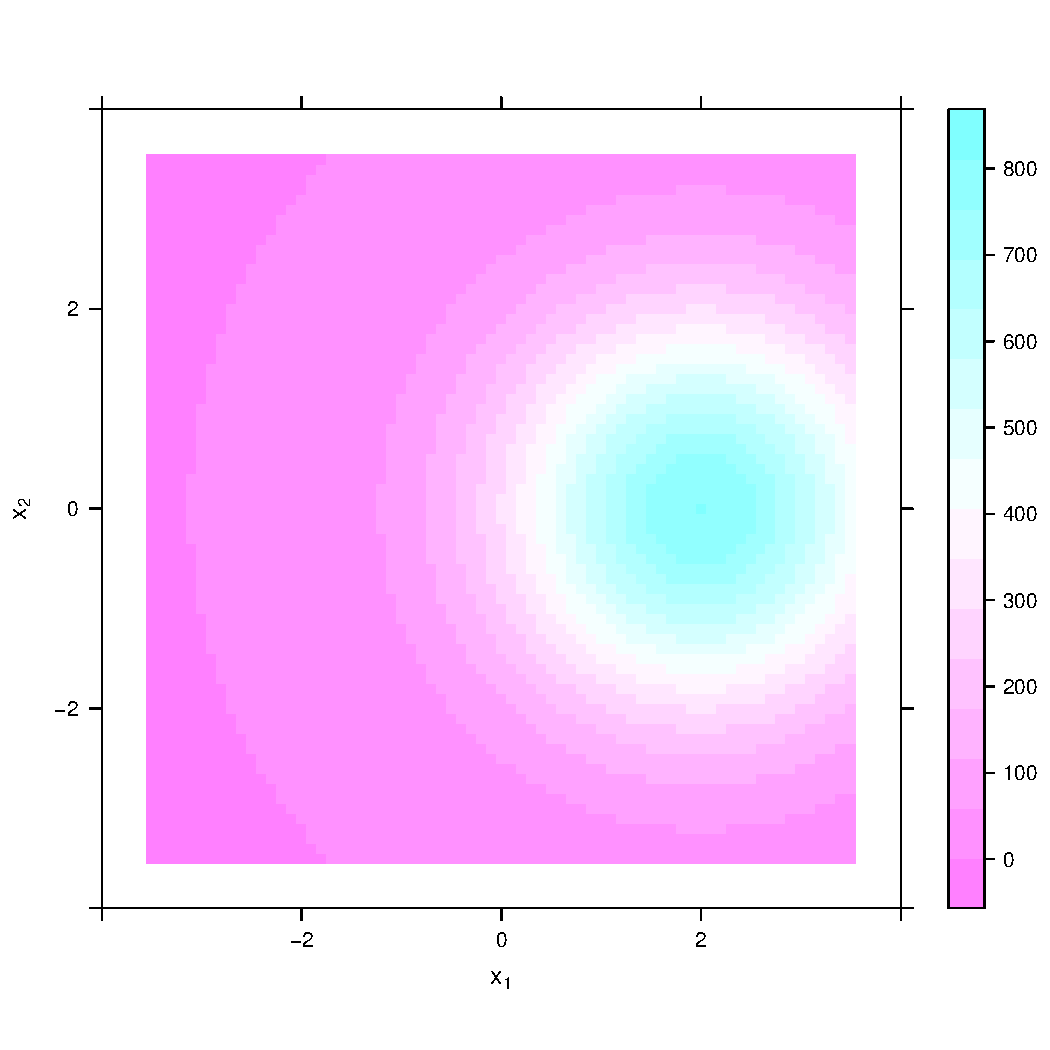
\includegraphics[width=\textwidth]{output/population-heatmap}
        \subcaption{Population distribution}
        \label{fig:cases_scatter:unif_100_1.0_1h:popdist}
    \end{subfigure}
    \begin{subfigure}[t]{0.32\textwidth}
        \includegraphics[width=\textwidth]{output/population-points}
        \subcaption{Population realization}
        \label{fig:cases_scatter:unif_100_1.0_1h:poppts}
    \end{subfigure}%
    \begin{subfigure}[t]{0.32\textwidth}
        \includegraphics[width=\textwidth]{output/population_and_incidents_scatter}
        \subcaption{With incidents}
        \label{fig:cases_scatter:unif_100_1.0_1h:incidentspts}
    \end{subfigure}%
    \caption[Example population and incidents: single-peak risk on uniform population]
        {Example population and incidents of one realization of single-peak risk of \glsentryname{factor} 100 with \glsentryname{spread} of 1.0 on a uniform population of 10,000. The red dots are the true peak. The blue diamonds are the peaks of the estimates. The black crosses are the centroid peaks of the estimates.}
    \label{fig:cases_scatter:unif_100_1.0_1h}    
\end{figure}

%%%%%%%%%%%%%%%%%%%%%%%%%%%%%%%%%%%%%%%%%%%%%%%%%
% Example cases heat map - unif_100_1.0_1h
%%%%%%%%%%%%%%%%%%%%%%%%%%%%%%%%%%%%%%%%%%%%%%%%%
\begin{figure}[htbp]
    \centering
    \begin{subfigure}[t]{0.45\textwidth}
        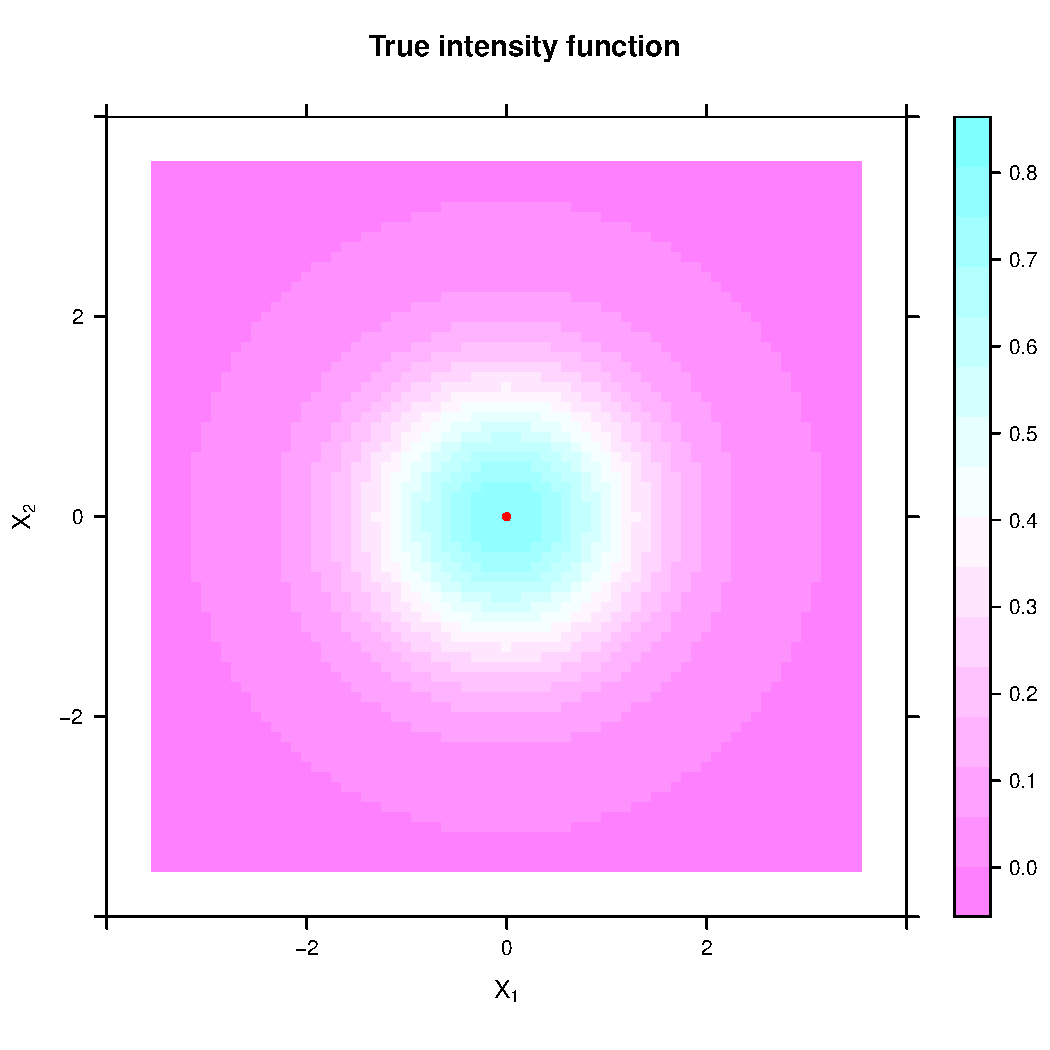
\includegraphics[width=\textwidth]{output/true_intensity_heatmap}
        \subcaption{True incident risk function}
        \label{fig:cases_heatmap:unif_100_1.0_1h:true}
    \end{subfigure}%
    \begin{subfigure}[t]{0.45\textwidth}
        \includegraphics[width=\textwidth]{output/oracle_intensity_heatmap}
        \subcaption{Incident risk estimate using Oracle bandwidth}
        \label{fig:cases_heatmap:unif_100_1.0_1h:oracle}
    \end{subfigure}

    \begin{subfigure}[b]{0.45\textwidth}
        \includegraphics[width=\textwidth]{output/silverman_intensity_heatmap}
        \subcaption{Incident risk estimate using Silverman bandwidth}
        \label{fig:cases_heatmap:unif_100_1.0_1h:silverman}
    \end{subfigure}%
    \begin{subfigure}[b]{0.45\textwidth}
        \includegraphics[width=\textwidth]{output/CV_intensity_heatmap}
        \subcaption{Incident risk estimate using Cross-validation bandwidth}
        \label{fig:cases_heatmap:unif_100_1.0_1h:cv}
    \end{subfigure}
    \caption[Example incidents: uniform incident risk on uniform population, 100 cases]
        {Example incidents: uniform incident risk on uniform population, 100 cases}
    \label{fig:cases_heatmap:unif_100_1.0_1h}
\end{figure}

In order to better understand the incident risk and the estimates,
we use a two-dimensional geographic heatmap of the study area \gls{W} to show a single simulation realization in
\cref{fig:cases_heatmap:unif_100_1.0_1h}.
The color of a point $\xvec$ represents the risk or estimated risk of an incident at that point.
\Cref{fig:cases_heatmap:unif_100_1.0_1h:true} shows a heatmap of the true distribution function.
We see the \gls{dkd} estimates obtained using the \gls{oracle} in \subref{fig:cases_heatmap:unif_100_1.0_1h:oracle},
\gls{silverman} in \subref{fig:cases_heatmap:unif_100_1.0_1h:silverman} and \gls{cv} in \subref{fig:cases_heatmap:unif_100_1.0_1h:cv}.
The red dot is the location of the true peak.
The blue diamond is the location of the estimated peak,
and the black cross is the location of the centroid estimated peak.

%%%%%%%%%%%%%%%%%%%%%%%%%%%%%%%%%%%%%%%%%%%%%%%%%
% Mean errors - unif_100_1.0_1h
%%%%%%%%%%%%%%%%%%%%%%%%%%%%%%%%%%%%%%%%%%%%%%%%%
\begin{table}[htbp]
    \centering
    % latex table generated in R 3.3.3 by xtable 1.8-2 package
% Mon Jan 15 21:47:29 2018
\begin{tabular}{lrrr}
  \hline
 & Oracle & Silverman & CV \\ 
  \hline
MISE & 0.000022 & 0.000035 & 0.000033 \\ 
  Relative MISE & 0.003402 & 0.005404 & 0.004996 \\ 
  Normalized MISE & 0.000022 & 0.000035 & 0.000033 \\ 
  MIAE & 0.002515 & 0.003126 & 0.003003 \\ 
  Relative MIAE & 0.031137 & 0.038695 & 0.037178 \\ 
  Max Error & 0.021087 & 0.031111 & 0.029319 \\ 
  Peak bias & -0.010671 & 0.006739 & 0.004427 \\ 
  Relative Peak bias & -0.132093 & 0.083426 & 0.054803 \\ 
  Peak drift & 0.288634 & 0.418493 & 0.401299 \\ 
  Relative Peak drift & 0.041233 & 0.059785 & 0.057328 \\ 
  Centroid bias & -0.011216 & -0.000155 & -0.001331 \\ 
  Relative Centroid bias & -0.138849 & -0.001917 & -0.016472 \\ 
  Centroid drift & 0.207657 & 0.222708 & 0.221023 \\ 
  Relative Centroid drift & 0.029665 & 0.031815 & 0.031575 \\ 
   \hline
\end{tabular}

    \caption{Mean error rates for uniform population, single-peak risk with \glsentryname{spread} 1.0 of \glsentryname{factor} 100}
    \label{tab:errors:unif_100_1.0_1h}
\end{table}

\Cref{tab:errors:unif_100_1.0_1h} contains a summary of all of the measures of accuracy for this experiment.
We can see that for most measures, the \gls{oracle} selected bandwidth provides the best results.
Since the \gls{oracle} bandwidth is designed to be approximate the \gls{mise}-optimal bandwidth \gls{h_opt},
this is not surprising.
However, in real world scenarios, the true function is unknown, and hence it is impossible to compute the \gls{oracle} bandwidth.
Therefore, we are interested in knowing how close the \gls{silverman} and \gls{cv} bandwidth selection methods can get to the \gls{oracle} for the different measures.
One exception is the \gls{peak bias}, which measures the difference between the maximum of the estimated risk and the maximum of the true risk (see \cref{subsec:method:peak_bias}).
In this experiment, the \gls{silverman} and \gls{cv} bandwidths produced lower absolute \gls{peak bias} values than the \gls{oracle}. 
However, the \gls{oracle} and \gls{cv} bandwidths resulted in negative biases,
which is what we expected,
since the process of smoothing generally lowers high values (peaks) and raises low values.
The \gls{silverman} bandwidth, on the other hand, produced a positive value,
which may indicate undersmoothing.
This requires further study.

In \cref{fig:ise:unif_100_1.0_1h}, we look at the distribution of the \gls{ise}.
As described in \cref{subsec:method:mise},
the \gls{iae} gives a summary of the error of the estimate over all of \gls{W},
that penalizes higher error values.
In particular, we see that the relative and normalized \gls{ise} have similarly shaped distributions, although the scale is different.
We also observe that the distributions are skewed to the right,
indicating that for this simple setup,
the accuracy of the \gls{dkd} for a specific sample is more likely to be below the \gls{mise}.
Finally, we note that the estimates calculated with \gls{silverman} and \gls{cv}
selected bandwidths and their corresponding mean values had similar performance in \gls{ise}.

%%%%%%%%%%%%%%%%%%%%%%%%%%%%%%%%%%%%%%%%%%%%%%%%%
% ISE distribution - unif_100_1.0_1h
%%%%%%%%%%%%%%%%%%%%%%%%%%%%%%%%%%%%%%%%%%%%%%%%%
\begin{figure}[htbp]
    \centering
    \begin{subfigure}[b]{0.45\textwidth}
        \includegraphics[width=\textwidth]{output/ise-relative-histogram}
        \subcaption{Relative \glsentryname{ise}}
    \end{subfigure}
    \begin{subfigure}[b]{0.45\textwidth}
        \includegraphics[width=\textwidth]{output/ise-normalized-histogram}
        \subcaption{Normalized \glsentryname{ise}}
    \end{subfigure}
    \caption[\glsentryname{ise}: Single-peak of 100 on uniform population]{\glsentryname{ise} density for a single-peak intensity with \glsentryname{spread} of 1.0 and \glsentryname{factor} of 100 on a uniform population. Vertical lines indicate the estimated \glsentryname{mise} of the simulations. \glsentryname{nmise} values are multiplied by $10^9$.}
    \label{fig:ise:unif_100_1.0_1h}
\end{figure}

%%%%%%%%%%%%%%%%%%%%%%%%%%%%%%%%%%%%%%%%%%%%%%%%%
% IAE distribution - unif_100_1.0_1h
%%%%%%%%%%%%%%%%%%%%%%%%%%%%%%%%%%%%%%%%%%%%%%%%%
\begin{figure}[htbp]
    \centering
    \begin{subfigure}[b]{0.45\textwidth}
        \includegraphics[width=\textwidth]{output/iae-relative-histogram}
        \subcaption{Relative \glsentryname{iae}}
    \end{subfigure}
    \begin{subfigure}[b]{0.45\textwidth}
        \includegraphics[width=\textwidth]{output/iae-normalized-histogram}
        \subcaption{Normalized \glsentryname{iae}}
    \end{subfigure}
    \caption[\glsentryname{iae}: Single-peak of 100 on uniform population]{\glsentryname{iae} density for a single-peak intensity with \glsentryname{spread} of 1.0 and \glsentryname{factor} of 100 on a uniform population. Vertical lines indicate the estimated \glsentryname{miae} of the simulations.}
    \label{fig:iae:unif_100_1.0_1h}
\end{figure}

%%%%%%%%%%%%%%%%%%%%%%%%%%%%%%%%%%%%%%%%%%%%%%%%%
% Max error distribution - unif_100_1.0_1h
%%%%%%%%%%%%%%%%%%%%%%%%%%%%%%%%%%%%%%%%%%%%%%%%%
\begin{figure}[htbp]
    \centering
    \includegraphics[width=0.45\textwidth]{output/maxerr-histogram}
    \caption[\glsentryname{supremum error}: Single-peak of 100 on uniform population]{\glsentryname{supremum error} density for a single-peak intensity with \glsentryname{spread} of 1.0 and \glsentryname{factor} of 100 on a uniform population. Vertical lines indicate the estimated mean \glsentryname{supremum error} of the simulations.}
    \label{fig:maxerr:unif_100_1.0_1h}
\end{figure}

\Cref{fig:ise:unif_100_1.0_1h} shows the relative and normalized distributions of the \gls{iae}.
As described in \cref{subsec:method:miae},
the \gls{iae} gives a summary of the error of the estimate over all of \gls{W},
giving equal weight to all error values.
Once again, the normalized and relative error measures have similar distributions.
The \gls{oracle} bandwidth selection technique is still notably more accurate when comparing with \gls{iae} than with \gls{ise}.
However, for \gls{iae} we see that \gls{cv} bandwidth selection results in a wider distribution than with \gls{silverman}.

In \cref{fig:maxerr:unif_100_1.0_1h}, we look at the distribution of the \gls{supremum error}.
As described in \cref{subsec:method:sup_error},
the \gls{supremum error} is the worst-case error of the estimate on \gls{W}.
We observe that the distributions are once again skewed to the right,
indicating that for this simple setup,
the worst-case accuracy of the \gls{dkd} for a specific sample is more likely to be below the average \gls{supremum error}.
Finally, we note that the estimates calculated with \gls{silverman} and \gls{cv}
selected bandwidths and their corresponding mean values had similar performance in \gls{supremum error}.


%%%%%%%%%%%%%%%%%%%%%%%%%%%%%%%%%%%%%%%%%%%%%%%%%
% Peaks - unif_100_1.0_1h
%%%%%%%%%%%%%%%%%%%%%%%%%%%%%%%%%%%%%%%%%%%%%%%%%
\begin{figure}[htbp]
    \centering
    \begin{subfigure}[b]{0.45\textwidth}
        \includegraphics[width=\textwidth]{output/peak-dist-histogram}
        \subcaption{Peak distance from truth}
        \label{fig:peaks:unif_100_1.0_1h:dist}
    \end{subfigure}
    \begin{subfigure}[b]{0.45\textwidth}
        \includegraphics[width=\textwidth]{output/peak-height-histogram}
        \subcaption{Peak height error}
        \label{fig:peaks:unif_100_1.0_1h:height}
    \end{subfigure}
    \caption[Peak accuracy: Single-peak of 100 on uniform population]{Peak accuracy measure densities for a single-peak intensity with \glsentryname{spread} of 1.0 and \glsentryname{factor} of 100 on a uniform population. Vertical lines indicate the mean values of the simulations.}
    \label{fig:peaks:unif_100_1.0_1h}
\end{figure}

%%%%%%%%%%%%%%%%%%%%%%%%%%%%%%%%%%%%%%%%%%%%%%%%%
% Centroids - unif_100_1.0_1h
%%%%%%%%%%%%%%%%%%%%%%%%%%%%%%%%%%%%%%%%%%%%%%%%%
\begin{figure}[htbp]
    \centering
    \begin{subfigure}[b]{0.45\textwidth}
        \includegraphics[width=\textwidth]{output/centroid-dist-histogram}
        \subcaption{Centroid peak distance from truth}
    \end{subfigure}
    \begin{subfigure}[b]{0.45\textwidth}
        \includegraphics[width=\textwidth]{output/centroid-height-histogram}
        \subcaption{Centroid peak height error}
    \end{subfigure}
    \caption[Centroid accuracy: Single-peak of 100 on uniform population]{Peak accuracy measures densitiesu sing centroid technique for a single-peak intensity with \glsentryname{spread} of 1.0 and \glsentryname{factor} of 100 on a uniform population. Vertical lines indicate the mean values of the simulations.}
    \label{fig:centroids:unif_100_1.0_1h}
\end{figure}

For both of the peak distance errors (\cref{fig:peaks:unif_100_1.0_1h:dist}) and peak height errors (\cref{fig:peaks:unif_100_1.0_1h:height}) of this experiment,
we see the \gls{cv} bandwidth selection outperforms the \gls{silverman} rule of thumb, and that the \gls{oracle} seems to outperform them both.
In fact, the \gls{peak bias}, which we estimate using the mean \gls{peak error},
is positive for \gls{silverman}.
This indicates a tendency towards undersmoothing.
We note that all three of bandwidth selection techniques are designed to minimize \gls{mise}.
We also note the multi-modal peak distance distributions.
We believe this is an artifact of the experimental design,
since our estimate of the peak will always be at one of a fixed, discrete number of points on a grid in the study area.

In \cref{fig:centroids:unif_100_1.0_1h} we see the distributions of \gls{peak error} and \gls{peak drift} using the centroid estimation technique.
We note that the scales of both types of error are markedly improved.
That is, the centroid technique improves both the estimated location and estimated height of the peak.

%%%%%%%%%%%%%%%%%%%%%%%%%%%%%%%%%%%%%%%%%%%%%%%%%
% Bandwidths - unif_100_1.0_1h
%%%%%%%%%%%%%%%%%%%%%%%%%%%%%%%%%%%%%%%%%%%%%%%%%
\begin{figure}[htbp]
    \centering
    \begin{subfigure}[t]{0.45\textwidth}
        \includegraphics[width=\textwidth]{output/bandwidths-x1}
        \subcaption{CV Bandwidths - $x_1$}
        \label{fig:bandwidths:unif_100_1.0_1h:x1}
    \end{subfigure}
    \begin{subfigure}[t]{0.45\textwidth}
        \includegraphics[width=\textwidth]{output/bandwidths-x2}
        \subcaption{CV Bandwidths - $x_2$}
        \label{fig:bandwidths:unif_100_1.0_1h:x2}
    \end{subfigure}

    \begin{subfigure}[t]{0.45\textwidth}
        \includegraphics[width=\textwidth]{output/bandwidths-difference}
        \subcaption{Difference between $x_1$ and $x_2$ bandwidths}
        \label{fig:bandwidths:unif_100_1.0_1h:diff}
    \end{subfigure}
    \begin{subfigure}[t]{0.45\textwidth}
        \includegraphics[width=\textwidth]{output/bandwidths-silverman}
        \subcaption{Silverman Bandwidths}
        \label{fig:bandwidths:unif_100_1.0_1h:silverman}
    \end{subfigure}
    \caption[Bandwidths: Single-peak of 100 on uniform population]{\glsentryname{cv} bandwidths: $x_1$, $x_2$ and difference and \glsentryname{silverman} bandwidth histograms for  a single-peak intensity with \glsentryname{spread} of 1.0 and \glsentryname{factor} of 100 on a uniform population}
    \label{fig:bandwidths:unif_100_1.0_1h}
\end{figure}

The bandwidths selected by \gls{cv} were allowed to vary in the $x_1$ and $x_2$ directions.
In \cref{fig:bandwidths:unif_100_1.0_1h:x1,fig:bandwidths:unif_100_1.0_1h:x2} we see that the distributions of these bandwidths observed in this experiment are quite similar,
while \cref{fig:bandwidths:unif_100_1.0_1h:diff} shows that they often differ significantly in the indidual realizations.
The distribution of the \gls{silverman} selected bandwidths is quite much more symmetric, and has a lower mean value (\cref{fig:bandwidths:unif_100_1.0_1h:silverman}).

% Restore graphics and input path
\graphicspath{{./}}
\makeatletter
\def\input@path{{./}}
\makeatother

%%%%%%%%%%%%%%%%%%%%%%%%%%%%%%%%%%%%%%%%%%%%%%%%%%%%%%%%%%%%%%%%%%%%%%%%%%%%%%
%%
%% Section: Effect of number of incidents with fixed population
%%
%%%%%%%%%%%%%%%%%%%%%%%%%%%%%%%%%%%%%%%%%%%%%%%%%%%%%%%%%%%%%%%%%%%%%%%%%%%%%%
\section[Effect of number of incidents with fixed population]
    {Effect of \glsentryname{factor} for a fixed, uniform population of 10,000 and single peak with \glsentryname{spread} 1.0}
\label{sec:results:number_of_incidents}

%%%%%%%%%%%%%%%%%%%%%%%%%%%%%%%%%%%%%%%%%%%%%%%%%
% Parameter table - expected number of incidents
%%%%%%%%%%%%%%%%%%%%%%%%%%%%%%%%%%%%%%%%%%%%%%%%%
\begin{table}[htbp]
    \centering
    \begin{tabular}{ll}
        \hline
        Parameter & Value \\
        \hline
        Population size & 10,000 \\
        Population \glsentryname{spread} & uniform \\
        Population center & uniform \\
        \Glsentryname{factor} & 50, 100, 200, 500, 1,000 \\
        Incident \glsentryname{spread} & 1.0 \\
        Incident center & (0,0) \\
        \hline
    \end{tabular}
    \caption[Effect of \glsentryname{factor} with fixed population]
        {Experimental parameter values varying \glsentryname{factor} for a fixed, uniform population of 10,000 and single peak with spread 1.0}
    \label{tab:params:results:number_of_incidents}
\end{table}

In this section we examine and compare the results of five experiments in which we vary the \glspl{factor}
of a single-peak risk function.
The unknown information that one is trying to discover, is the risk of a person catching a specific disease over a defined time period.
This is analogous to a real-world researcher combining the several years worth of incident data from the same population.
Our question is, will this lead to more accurate results for the \gls{dkd}?
We keep the population size constant at 10,000, distributed uniformly throughout the study area.
The risk function for each of the five experiments has a single peak,
centered at the origin,
with a \gls{spread} of 1.0.
The \glspl{factor} used in the experiments in this section were 50, 100, 200, 500, and 1,000.
The full set of accuracy measures for these cases can be found in \cref{tab:mean_error_rates:unif_50_1.0_1h,tab:mean_error_rates:unif_100_1.0_1h,tab:mean_error_rates:unif_200_1.0_1h,tab:mean_error_rates:unif_500_1.0_1h,tab:mean_error_rates:unif_1000_1.0_1h} in \autoref{ch:results_tables}.
We note that as in \cref{sec:results:unif_100_1.0_1h}, the \gls{peak bias} values were positive for the \gls{silverman} bandwidth based estimates.
\autoref{fig:one_sample:unif_NCases_1h} shows how one realization of incidents, distributed over the population, for sample sizes of 100 and 500.

%%%%%%%%%%%%%%%%%%%%%%%%%%%%%%%%%%%%%%%%%%%%%%%%%
% Examples showing factorS
%%%%%%%%%%%%%%%%%%%%%%%%%%%%%%%%%%%%%%%%%%%%%%%%%
\begin{figure}[htbp]
    \centering
    \begin{subfigure}{0.45\textwidth}
        \includegraphics[width=\textwidth]{results/unif_100_1.0_1h/output/population_and_incidents_scatter}
        \caption{100 incidents}
    \end{subfigure}
    \begin{subfigure}{0.45\textwidth}
        \includegraphics[width=\textwidth]{results/unif_500_1.0_1h/output/population_and_incidents_scatter}
        \caption{500 incidents}
    \end{subfigure}
        \caption{A single realization of different \glspl{factor} from a single-peak risk on a uniform population}
        \label{fig:one_sample:unif_NCases_1h}
\end{figure}

According to the theory developed in \cref{sec:theory:bandwidth},
the bandwidth should decrease as the \textit{observed} sample size increases according to the formula

\begin{equation}
    \label{eq:h_opt}
    \gls{h_opt} = O(n^{-\frac{1}{6}}) \text{.}
\end{equation}

\Cref{tab:results:bandwidth_vs_mu} compares the selected bandwidths and \gls{nmise} obtained for different \glspl{factor},
since this is the variable which we control.
We observe that all of the bandwidths decrease as \gls{mu} increases.
When there is a power relationship as in \cref{eq:h_opt} above, we can take the logarithm of both variables to produce a linear relationship.
The slope of the line in the log-log equation is equal to the power of the original equation.
\Cref{fig:results:bandwidth_by_incidents} shows log-log plots of the observed bandwidths that were obtained by the various selection mechanisms.
We have fit a line to each plot to show the linear relationship in the log-log equations, and hence the power relationship between the bandwidths selected by the different mechanisms and the sample size, represented by \gls{factor}.
The observed values for the power of $n$ as represented by $N_I$ are shown in \cref{tab:results:bandwidth_alpha_by_selector}.

% latex table generated in R 3.3.3 by xtable 1.8-2 package
% Sun Mar 11 17:51:17 2018
\begin{table}[ht]
\centering
\begin{tabular}{rrrrrrr}
  \hline
$\mu$ & $h_{o}(x_1)$ & $h_{o}(x_2)$ & $h_{s}$ & Oracle NMISE & Silverman NMISE & CV NMISE \\ 
  \hline
50.00 & 1.50 & 1.50 & 1.03 & 3.54 & 5.72 & 5.44 \\ 
  100.00 & 1.30 & 1.40 & 0.92 & 2.22 & 3.53 & 3.40 \\ 
  200.00 & 1.20 & 1.20 & 0.82 & 1.32 & 2.09 & 1.99 \\ 
  500.00 & 1.10 & 1.00 & 0.70 & 0.68 & 1.07 & 0.96 \\ 
  1000.00 & 0.90 & 0.90 & 0.63 & 0.38 & 0.62 & 0.54 \\ 
   \hline
\end{tabular}
\caption[Bandwidth and accuracy by number of incidents]{Bandwidth and accuracy by number of incidents for uniform population of 10,000 with single-peak risk function, spread of 1.0. The NMISE values are scaled by $10^9$.} 
\label{tab:results:bandwidth_vs_mu}
\end{table}


%latex.default(df.alpha, file = "alpha_by_selector.tex", title = "alpha_by_selector",     where = "htbp", label = "tab:results:bandwidth_alpha_by_selector",     rowname = NULL, cdec = c(0, 3), caption.loc = "bottom", caption = "Bandwidth onvergence rate $\\alpha$ of for different bandwidth selectors for a single-peak risk function with spread of 1.0 on a uniform population of 10,000.",     caption.lot = "Bandwidth convergence rate of bandwidth selectors")%
\begin{table}[htbp]
\begin{center}
\begin{tabular}{lr}
\hline\hline
\multicolumn{1}{c}{Selector}&\multicolumn{1}{c}{Slope}\tabularnewline
\hline
Oracle Bandwidth $x_1$&$-0.156$\tabularnewline
Oracle Bandwidth $x_1$&$-0.179$\tabularnewline
Silverman&$-0.167$\tabularnewline
CV Bandwidth $x_1$&$-0.171$\tabularnewline
CV Bandwidth $x_2$&$-0.205$\tabularnewline
Theory&$-0.167$\tabularnewline
\hline
\end{tabular}
\caption[Bandwidth convergence rate of bandwidth selectors]{Bandwidth onvergence rate $\alpha$ of for different bandwidth selectors for a single-peak risk function with spread of 1.0 on a uniform population of 10,000.\label{tab:results:bandwidth_alpha_by_selector}}\end{center}
\end{table}


%%%%%%%%%%%%%%%%%%%%%%%%%%%%%%%%%%%%%%%%%%%%%%%%%
% Selected bandwidty by factor
%%%%%%%%%%%%%%%%%%%%%%%%%%%%%%%%%%%%%%%%%%%%%%%%%
\begin{figure}[htbp]
    \centering
    \begin{subfigure}[t]{0.195\textwidth}
        \centering
        \includegraphics[width=\textwidth]{results/by_h_per_mu/oracle_bandwidth_x1_vs_mu.pdf}
        \subcaption{Oracle bandwidth in $x_1$ direction by \glsentryname{factor}}
    \end{subfigure}
    \begin{subfigure}[t]{0.195\textwidth}
        \centering
        \includegraphics[width=\textwidth]{results/by_h_per_mu/oracle_bandwidth_x2_vs_mu.pdf}
        \subcaption{Oracle bandwidth in $x_2$ direction by \glsentryname{factor}}
    \end{subfigure}
    \begin{subfigure}[t]{0.195\textwidth}
        \centering
        \includegraphics[width=\textwidth]{results/by_h_per_mu/silverman_bandwidth_vs_mu.pdf}
        \subcaption{Mean Silverman bandwidth by \glsentryname{factor}}
    \end{subfigure}
    \begin{subfigure}[t]{0.195\textwidth}
        \centering
        \includegraphics[width=\textwidth]{results/by_h_per_mu/cv_bandwidth_x1_vs_mu.pdf}
        \subcaption{Mean CV bandwidth in $x_1$ direction by \glsentryname{factor}}
    \end{subfigure}
    \begin{subfigure}[t]{0.195\textwidth}
        \centering
        \includegraphics[width=\textwidth]{results/by_h_per_mu/cv_bandwidth_x2_vs_mu.pdf}
        \subcaption{Mean CV bandwidth in $x_2$ direction by \glsentryname{factor}}
    \end{subfigure}
    \caption[Selected bandwidth by \glsentryname{factor}]
        {Log-log plot of selected bandwidth by \glsentryname{factor} for different bandwidth selectors.
        The slope of the log-log plot indicates the power of $n$ in the convergence rate.}
    \label{fig:results:bandwidth_by_incidents}    
\end{figure}

%%%%%%%%%%%%%%%%%%%%%%%%%%%%%%%%%%%%%%%%%%%%%%%%%
% MISE by number of cases
%%%%%%%%%%%%%%%%%%%%%%%%%%%%%%%%%%%%%%%%%%%%%%%%%
\begin{figure}[htbp]
    \centering
    \begin{subfigure}[b]{0.24\textwidth}
        \includegraphics[width=\textwidth]{results/by_num_cases/MISE-vs-cases}
        \subcaption{\glsentryname{mise}}
        \label{fig:ise:unif_NCases_1h:mise}
    \end{subfigure}
    \begin{subfigure}[b]{0.24\textwidth}
        \includegraphics[width=\textwidth]{results/by_num_cases/RMISE-vs-cases}
        \subcaption{\glsentryname{rmise}}
        \label{fig:ise:unif_NCases_1h:rmise}
    \end{subfigure}
    \begin{subfigure}[b]{0.24\textwidth}
        \includegraphics[width=\textwidth]{results/by_num_cases/NMISE-vs-cases}
        \subcaption{\glsentryname{nmise}}
        \label{fig:ise:unif_NCases_1h:nmise}
    \end{subfigure}
    \begin{subfigure}[b]{0.24\textwidth}
        \includegraphics[width=\textwidth]{results/by_num_cases/NMISE-vs-cases-log-log}
        \subcaption{\glsentryname{nmise} log-log}
        \label{fig:ise:unif_NCases_1h:nmise_log_log}
    \end{subfigure}
    \caption[\glsentryname{mise}: by number of cases]{\glsentryname{mise} vs. number of cases}
    \label{fig:ise:unif_NCases_1h}
\end{figure}

\autoref{fig:ise:unif_NCases_1h} shows the effect of \gls{factor} on the \gls{mise}, \gls{rmise} and on \gls{nmise}:
\autoref{fig:ise:unif_NCases_1h:mise} shows how \gls{mise} increases with \gls{factor}.
One might expect the error to associated with estimating a function to \textit{decrease} as the \gls{factor} increases.
However, the \gls{factor} increases linearly with the intensity function value.
For example, double the number of incidents corresponds to an intensity of twice the value.
This makes comparing the \gls{mise} of estimates of intensity functions difficult,
as the errors will also rise in the same direction.
In order to facilitate the comparison of intensity functions that have different expected number of incidents,
we use the \gls{rmise}and \gls{nmise}.
\Cref{fig:ise:unif_NCases_1h:rmise,fig:ise:unif_NCases_1h:nmise} shows how \gls{rmise} and \gls{nmise} decreases with \gls{factor}.
To test if there is a power relationship between \gls{nmise} and \gls{factor},
we take the logarithms of each variable and fit a line.
\autoref{fig:ise:unif_NCases_1h:nmise_log_log} is a log-log graph,
showing the linear relationship between the logarithm of \gls{nmise} and the logarithm of the \gls{factor}.
This indicates a power relationship between \gls{nmise} and \gls{factor} for each bandwidth selection method is shown in \cref{tab:results:nmise_convergence_by_num_cases}.
They are all near to $-0.75$.

%latex.default(df.alpha, title = "nmise_convergence_table", where = "htbp",     label = "tab:results:nmise_convergence_by_sample_size", rowname = NULL,     cdec = c(0, 3), caption.loc = "bottom", caption = "NMISE convergence rate by sample size for different bandwidth selectors for a fixed, single-peak risk function with expected number of incidents 100 on a uniform population.",     caption.lot = "NMISE Convergence rate by sample size")%
\begin{table}[htbp]
\begin{center}
\begin{tabular}{lr}
\hline\hline
\multicolumn{1}{c}{Selector}&\multicolumn{1}{c}{Slope}\tabularnewline
\hline
Oracle&$-2.689$\tabularnewline
Silverman&$-2.688$\tabularnewline
CV&$-2.741$\tabularnewline
\hline
\end{tabular}
\caption[NMISE Convergence rate by sample size]{NMISE convergence rate by sample size for different bandwidth selectors for a fixed, single-peak risk function with expected number of incidents 100 on a uniform population.\label{tab:results:nmise_convergence_by_sample_size}}\end{center}
\end{table}



%%%%%%%%%%%%%%%%%%%%%%%%%%%%%%%%%%%%%%%%%%%%%%%%%%%%%%%%%%%%%%%%%%%%%%%%%%%%%%
%%
%% Section: Effect of risk spread with fixed population
%%
%%%%%%%%%%%%%%%%%%%%%%%%%%%%%%%%%%%%%%%%%%%%%%%%%%%%%%%%%%%%%%%%%%%%%%%%%%%%%%
\section[Effect of risk spread with fixed population]
    {Effect of risk \glsentryname{spread} for a fixed, uniform population of 10,000 and single peak with \glsentryname{spread} 1.0}
\label{sec:results:spread}

%%%%%%%%%%%%%%%%%%%%%%%%%%%%%%%%%%%%%%%%%%%%%%%%%
% Parameter table - spread
%%%%%%%%%%%%%%%%%%%%%%%%%%%%%%%%%%%%%%%%%%%%%%%%%
\begin{table}[htbp]
    \centering
    \begin{tabular}{ll}
        \hline
        Parameter & Value \\
        \hline
        Population size & 10,000 \\
        Population \glsentryname{spread} & uniform \\
        Population center & uniform \\
        \Glsentryname{factor} & 100 \\
        Incident \glsentryname{spread} & 0.7, 1.0, 1.4, 2.0, 2.8 \\
        Incident center & (0,0) \\
        \hline
    \end{tabular}
    \caption[Effect of spread with fixed population]
        {Experimental parameter values varying \glsentryname{spread} for a fixed, uniform population of 10,000 and single peak with \glsentryname{spread} 1.0}
    \label{tab:params:results:spread}
\end{table}

In this section we examine and compare the results of five experiments in which we vary the \gls{spread} \gls{sigma_i}
of a single-peak risk function.
The unknown information that one is trying to discover is, how far away from a source of disease risk is safe.
Our question is, under different \glspl{spread}, how accurate is the \gls{dkd}?
Differing \glspl{spread} are analogous to different levels of concentration of the risk of disease is in a specific location.
Another way to look at it is, is how quickly the risk dissipates in space as one moves further away from a single source of disease risk.
We keep the population size constant at 10,000, distributed uniformly throughout the study area.
The risk function for each of the five experiments has a single peak,
centered at the origin,
with a \gls{factor} of 100.
The values of \gls{sigma_i} used in the experiments in this section are 0.7, 1.0, 1.4, 2.0, and 2.8.
The full set of accuracy measures for these cases can be found in \autoref{tab:mean_error_rates:unif_100_0.7_1h}, \autoref{tab:mean_error_rates:unif_100_1.0_1h}, \autoref{tab:mean_error_rates:unif_100_1.4_1h}, \autoref{tab:mean_error_rates:unif_100_2.0_1h}, and \autoref{tab:mean_error_rates:unif_100_2.8_1h} in \autoref{ch:results_tables}.
We note that as in \cref{sec:results:unif_100_1.0_1h}, the \gls{peak bias} values were positive for the \gls{silverman} bandwidth based estimates.
\autoref{fig:one_sample:unif_Spreads_1h} shows how one realization of incidents, distributed over the population, for \glspl{spread} of 1.0 and 2.8.

%%%%%%%%%%%%%%%%%%%%%%%%%%%%%%%%%%%%%%%%%%%%%%%%%
% Examples showing spreads
%%%%%%%%%%%%%%%%%%%%%%%%%%%%%%%%%%%%%%%%%%%%%%%%%
\begin{figure}[htbp]
    \centering
    \begin{subfigure}{0.45\textwidth}
        \includegraphics[width=\textwidth]{results/unif_100_1.0_1h/output/population_and_incidents_scatter}
        \caption{\Glsentryname{spread} of 1.0}
    \end{subfigure}
    \begin{subfigure}{0.45\textwidth}
        \includegraphics[width=\textwidth]{results/unif_100_2.8_1h/output/population_and_incidents_scatter}
        \caption{\Glsentryname{spread} of 2.8}
    \end{subfigure}
    \caption{A single realization of different \glspl{spread} from a single-peak risk on a uniform population}
    \label{fig:one_sample:unif_Spreads_1h}
\end{figure}

The effect of increasing \gls{spread} is that the peak of the risk function becomes less pronounced.
The incidents that are generated by the corresponding \gls{spp} are distributed more evenly and widely throughout the study area \gls{W},
as can be seen in \cref{fig:one_sample:unif_Spreads_1h}.
We observe the effect of varying \gls{sigma_i} on the selected bandwidths.
The \gls{oracle}, \gls{silverman}, and \gls{cv} bandwidths all increase as the spread increases, as can be seen in \cref{tab:results:bandwidth_vs_spread}.
This is to be expected, since smaller bandwidths result in decreased smoothing,
which is necessary when the true risk function varies more quickly as is the case with smaller \gls{sigma_i} values.
We note that the \gls{cv} selected bandwidths are closer to \gls{h_opt} as approximated by the \gls{oracle}, than are the \gls{silverman} bandwidths.

% latex table generated in R 3.3.3 by xtable 1.8-2 package
% Sun Mar 11 18:06:07 2018
\begin{table}[ht]
\centering
\begin{tabular}{lrrrrrr}
  \hline
$\sigma_i$ & $h_{o}(x_1)$ & $h_{o}(x_2)$ & $h_{s}$ & Oracle NMISE & Silverman NMISE & CV NMISE \\ 
  \hline
0.7 & 0.90 & 1.00 & 0.64 & 4.15 & 6.98 & 6.67 \\ 
  1.0 & 1.30 & 1.40 & 0.92 & 2.22 & 3.53 & 3.40 \\ 
  1.4 & 1.90 & 1.80 & 1.26 & 1.16 & 1.87 & 1.64 \\ 
  2.0 & 2.50 & 2.60 & 1.55 & 0.64 & 1.19 & 0.92 \\ 
   \hline
\end{tabular}
\caption[Bandwidth and accuracy by spread of incidents]{Bandwidth and accuracy by spread for uniform population of 10,000 with single-peak risk function with expected number of incidents 100. The NMISE values are scaled by $10^9$.} 
\label{tab:results:bandwidth_vs_mu}
\end{table}


We also observe that the \gls{nmise} decreases significantly with increasing \gls{sigma_i}.
This provides evidence that the \gls{dkd} may be better suited to situations where the true underlying risk is smoother.
In \cref{fig:ise:unif_Spreads_1h} take a closer look at the distributions of \gls{mise}, \gls{rmise}, and \gls{nmise}.
\textbf{What we see is that as \gls{sigma_i} increases, both absolute and normalized \gls{mise} decrease but relative \gls{mise} increases.}
This is the same for all bandwidth selection methods.
Since we keep \gls{mu} constant throughout the experiment, it would make sense absolute and normalized \gls{mise} behave similarly.
The \gls{rmise} takes a local view of relative error, and here we see that as the \gls{spread} increase, the \gls{mise} decreases but at a slower rate than the true function.


%%%%%%%%%%%%%%%%%%%%%%%%%%%%%%%%%%%%%%%%%%%%%%%%%
% MISE by spread
%%%%%%%%%%%%%%%%%%%%%%%%%%%%%%%%%%%%%%%%%%%%%%%%%
\begin{figure}[htbp]
    \centering
    \begin{subfigure}[t]{0.24\textwidth}
        \includegraphics[width=\textwidth]{results/by_cases_spread/MISE-vs-risk-spread}
        \caption{\glsentryname{mise}}
        \label{fig:ise:unif_Spreads_1h:mise}
    \end{subfigure}
    \begin{subfigure}[t]{0.24\textwidth}
        \includegraphics[width=\textwidth]{results/by_cases_spread/RMISE-vs-risk-spread}
        \caption{\glsentryname{rmise}}
        \label{fig:ise:unif_Spreads_1h:rmise}
    \end{subfigure}
    \begin{subfigure}[t]{0.24\textwidth}
        \includegraphics[width=\textwidth]{results/by_cases_spread/NMISE-vs-risk-spread}
        \caption{\glsentryname{nmise}}
        \label{fig:ise:unif_Spreads_1h:nmise}
    \end{subfigure}
    \begin{subfigure}[t]{0.24\textwidth}
        \includegraphics[width=\textwidth]{results/by_cases_spread/NMISE-vs-risk-spread-log-log}
        \caption{\glsentryname{nmise} log-log}
        \label{fig:ise:unif_Spreads_1h:nmise_log_log}
    \end{subfigure}
    \caption[\glsentryname{mise}: by risk \glsentryname{spread}]
        {The effect of \glsentryname{spread} on \glsentryname{mise} for different bandwidth selectors for a single-peak risk function with \gls{factor} 100 on a uniform population of 10,000}
    \label{fig:ise:unif_Spreads_1h}
\end{figure}

We look now at the asymptotic behavior of \gls{nmise} as $\gls{sigma_i} \to \infty$.
From \cref{fig:ise:unif_Spreads_1h:nmise_log_log} we see a polynomial relationship between \gls{nmise} and \gls{sigma_i} (\cref{eq:nmise:spread}).
\Cref{tab:results:nmise_convergence_by_cases_spread} shows the slope $\alpha_S$ that we observed for each bandwidth selection method.

\begin{equation}
    \label{eq:nmise:spread}
    \gls{nmise} = O(n^{\alpha_S})
\end{equation}
%latex.default(df.alpha, title = "nmise_convergence_table", where = "htbp",     label = "tab:results:nmise_convergence_by_sample_size", rowname = NULL,     cdec = c(0, 3), caption.loc = "bottom", caption = "NMISE convergence rate by sample size for different bandwidth selectors for a fixed, single-peak risk function with expected number of incidents 100 on a uniform population.",     caption.lot = "NMISE Convergence rate by sample size")%
\begin{table}[htbp]
\begin{center}
\begin{tabular}{lr}
\hline\hline
\multicolumn{1}{c}{Selector}&\multicolumn{1}{c}{Slope}\tabularnewline
\hline
Oracle&$-2.689$\tabularnewline
Silverman&$-2.688$\tabularnewline
CV&$-2.741$\tabularnewline
\hline
\end{tabular}
\caption[NMISE Convergence rate by sample size]{NMISE convergence rate by sample size for different bandwidth selectors for a fixed, single-peak risk function with expected number of incidents 100 on a uniform population.\label{tab:results:nmise_convergence_by_sample_size}}\end{center}
\end{table}


%%%%%%%%%%%%%%%%%%%%%%%%%%%%%%%%%%%%%%%%%%%%%%%%%%%%%%%%%%%%%%%%%%%%%%%%%%%%%%
%%
%% Section: Varying the sample size for fixed intensity
%%
%%%%%%%%%%%%%%%%%%%%%%%%%%%%%%%%%%%%%%%%%%%%%%%%%%%%%%%%%%%%%%%%%%%%%%%%%%%%%%
\section{Varying the population and sample size for fixed intensity}
\label{sec:results:unifNpop_1h}

%%%%%%%%%%%%%%%%%%%%%%%%%%%%%
% Parameter table
%%%%%%%%%%%%%%%%%%%%%%%%%%%%%
\begin{table}[htbp]
    \centering
    \begin{tabular}{ll}
        \hline
        Parameter & Value \\
        \hline
        Population size & 5,000, 10,000, 20,000, 50,000, 100,000 \\
        Population \gls{spread} & uniform \\
        Population center & uniform \\
        \Gls{factor} & 50, 100, 200, 500, 1000 \\
        Incident \gls{spread} & 1.0 \\
        Incident center & (0,0) \\
        \hline
    \end{tabular}
    \caption{Parameters used for varying the sample size for fixed intensity}
    \label{tab:params:unifNpop_1h}
\end{table}

We next examine the effect of increasing the sample size, while keeping the risk intensity function fixed.
Unlike what we did in \cref{sec:results:number_of_incidents} where we fixed the size of the population and allowed the risk function to change,
here we fix the risk function and change the population size.
This is analogous to increasing the size of the population under study, for example by increasing the study area.
In order to do this, we increase the population size and the \gls{factor} proportionately.
For example, in one experiment \gls{factor} is 50 and the population is 5,000,
and in the next experiment the \gls{factor} is 100 and the population is 10,000.
For this set of experiments, the population is uniformly distributed and the risk intensity has a single peak in the center with a fixed \gls{sigma_i} of 1.0.
Mean and standard deviations of accuracy measures for the experiments of this section are found in \cref{tab:mean_error_rates:unif5k_50_1.0_1h,tab:mean_error_rates:unif10k_100_1.0_1h,tab:mean_error_rates:unif20k_200_1.0_1h,tab:mean_error_rates:unif50k_500_1.0_1h,tab:mean_error_rates:unif100k_1000_1.0_1h}.

\Cref{fig:one_sample:unifNpop_1h} shows the denser population, as represented by the blue dots, and the larger sample size, represented by the red dots.
In both cases, the population is distributed uniformly throughout the study area,
while the incident samples are concentrated around the peak in the center.

%%%%%%%%%%%%%%%%%%%%%%%%%%%%%%%%%%%%%%%%%%%%%%%%%
% Examples showing sample size
%%%%%%%%%%%%%%%%%%%%%%%%%%%%%%%%%%%%%%%%%%%%%%%%%
\begin{figure}[htbp]
    \centering
    \begin{subfigure}{0.45\textwidth}
        \includegraphics[width=\textwidth]{results/unif10k_100_1.0_1h/output/population_and_incidents_scatter}
        \caption{100 incidents from population of 10,000}
    \end{subfigure}
    \begin{subfigure}{0.45\textwidth}
        \includegraphics[width=\textwidth]{results/unif50k_500_1.0_1h/output/population_and_incidents_scatter}
        \caption{500 incidents from population of 50,000}
    \end{subfigure}
    \caption{A single realization of different sample sizes from a single-peak risk on a uniform population, obtained by varying the \gls{factor} and population size in tandem while keeping the risk function $\lambda \xvec$ fixed}
    \label{fig:one_sample:unifNpop_1h}
\end{figure}

%%%%%%%%%%%%%%%%%%%%%%%%%%%%%%%%%%%%%%%%%%%%%%%%%
% MISE by sample + population
%%%%%%%%%%%%%%%%%%%%%%%%%%%%%%%%%%%%%%%%%%%%%%%%%
\begin{figure}[htbp]
    \centering
    \begin{subfigure}[b]{0.24\textwidth}
        \includegraphics[width=\textwidth]{results/by_pop_size/MISE-vs-population}
        \caption{\glsentryname{mise}}
        \label{fig:ise:unifNpop_1h:mise}
    \end{subfigure}
    \begin{subfigure}[b]{0.24\textwidth}
        \includegraphics[width=\textwidth]{results/by_pop_size/RMISE-vs-population}
        \caption{\glsentryname{rmise}}
        \label{fig:ise:unifNpop_1h:rmise}
    \end{subfigure}
    \begin{subfigure}[b]{0.24\textwidth}
        \includegraphics[width=\textwidth]{results/by_pop_size/NMISE-vs-population}
        \caption{\glsentryname{nmise}}
        \label{fig:ise:unifNpop_1h:nmise}
    \end{subfigure}
    \begin{subfigure}[b]{0.24\textwidth}
        \includegraphics[width=\textwidth]{results/by_pop_size/NMISE-vs-population-log-log}
        \caption{\glsentryname{nmise} log-log}
        \label{fig:ise:unifNpop_1h:nmise_log_log}
    \end{subfigure}
    \caption[\glsentryname{mise}: by sample and population size]{\glsentryname{mise} vs. sample and population size}
    \label{fig:ise:unifNpop_1h}
\end{figure}

In \cref{fig:ise:unifNpop_1h:mise} we see that in this experiment,
\gls{mise} decreases when the sample and population sizes increase.
\Gls{rmise} also decreases in a similar manner, as shown in \cref{fig:ise:unifNpop_1h:rmise}.
When we look at \cref{fig:ise:unifNpop_1h:nmise} we see that the rate of decrease of \gls{nmise} appears to be much higher than \gls{mise}.
In \cref{tab:results:nmise_convergence_by_sample_size} we see that when we fix the risk function $\lambda \xvec$,
the \gls{nmise} converges at a much higher rate than we observed in \cref{sec:results:number_of_incidents}.
We also note that selected the bandwidth using \gls{cv} appears to result in a slightly faster rate of convergence than \gls{silverman}.

%latex.default(df.alpha, title = "nmise_convergence_table", where = "htbp",     label = "tab:results:nmise_convergence_by_sample_size", rowname = NULL,     cdec = c(0, 3), caption.loc = "bottom", caption = "NMISE convergence rate by sample size for different bandwidth selectors for a fixed, single-peak risk function with expected number of incidents 100 on a uniform population.",     caption.lot = "NMISE Convergence rate by sample size")%
\begin{table}[htbp]
\begin{center}
\begin{tabular}{lr}
\hline\hline
\multicolumn{1}{c}{Selector}&\multicolumn{1}{c}{Slope}\tabularnewline
\hline
Oracle&$-2.689$\tabularnewline
Silverman&$-2.688$\tabularnewline
CV&$-2.741$\tabularnewline
\hline
\end{tabular}
\caption[NMISE Convergence rate by sample size]{NMISE convergence rate by sample size for different bandwidth selectors for a fixed, single-peak risk function with expected number of incidents 100 on a uniform population.\label{tab:results:nmise_convergence_by_sample_size}}\end{center}
\end{table}


%%%%%%%%%%%%%%%%%%%%%%%%%%%%%%%%%%%%%%%%%%%%%%%%%%%%%%%%%%%%%%%%%%%%%%%%%%%%%%
%%
%% Section: Varying the spread of the population density
%%
%%%%%%%%%%%%%%%%%%%%%%%%%%%%%%%%%%%%%%%%%%%%%%%%%%%%%%%%%%%%%%%%%%%%%%%%%%%%%%
\section{Varying the spread of the population density}
\label{sec:results:pSD_100_1h}

In this section, we compare the effect of different population distributions on the estimation of a single, fixed risk function.
The population s
The risk function has an \gls{factor} of 100.

\begin{table}[htbp]
\centering
% latex table generated in R 3.4.3 by xtable 1.8-2 package
% Tue Apr 03 11:15:13 2018
\begin{tabular}{lrrr}
  \hline
 & Oracle & Silverman & CV \\ 
  \hline
MISE & 0.001480 & 0.001468 & 0.001755 \\ 
  Relative MISE & 0.226751 & 0.224963 & 0.268930 \\ 
  Normalized MISE & 147.969414 & 146.802375 & 175.493859 \\ 
  MIAE & 0.006271 & 0.006336 & 0.006678 \\ 
  Relative MIAE & 0.077623 & 0.078435 & 0.082665 \\ 
  Normalized MIAE & 0.000063 & 0.000063 & 0.000067 \\ 
  Max Error & 0.405078 & 0.434458 & 0.405401 \\ 
  Normalized Max Error & 0.004051 & 0.004345 & 0.004054 \\ 
  Peak bias & 0.331304 & 0.360895 & 0.330921 \\ 
  Relative Peak bias & 4.101243 & 4.467549 & 4.096503 \\ 
  Peak drift & 2.223677 & 2.215194 & 2.274708 \\ 
  Relative Peak drift & 0.317668 & 0.316456 & 0.324958 \\ 
  Centroid bias & -0.008225 & -0.006728 & -0.011830 \\ 
  Relative Centroid bias & -0.101821 & -0.083283 & -0.146446 \\ 
  Centroid drift & 0.325701 & 0.299465 & 0.400859 \\ 
  Relative Centroid drift & 0.046529 & 0.042781 & 0.057266 \\ 
   \hline
\end{tabular}

\caption{Error rates for uniform population of 10,000, single peak intensity of \gls{factor} 100 and \gls{spread} 0.7}
\label{tab:results:p0.7_100_1.0_1h}
\end{table}


\begin{figure}[htbp]
    \centering
    \begin{subfigure}[b]{0.3\textwidth}
    \includegraphics[width=\textwidth]{results/by_population_spread/MISE-vs-population-spread}
    \caption{MISE}
    \end{subfigure}
    \begin{subfigure}[b]{0.3\textwidth}
    \includegraphics[width=\textwidth]{results/by_population_spread/RMISE-vs-population-spread}
    \caption{Relative MISE}
    \end{subfigure}
    \begin{subfigure}[b]{0.3\textwidth}
    \includegraphics[width=\textwidth]{results/by_population_spread/RMISE-vs-population-spread-log-log}
    \caption{Relative MISE log-log}
    \end{subfigure}
    \caption[MISE: by risk spread]{Mean Integrated Squared Error vs. population spread}
    \label{fig:ise:pSD_100_1h}
\end{figure}


%%%%%%%%%%%%%%%%%%%%%%%%%%%%%%%%%%%%%%%%%%%%%%%%%%%%%%%%%%%%%%%%%%%%%%%%%%%%%%
%%
%% Section: Distance between two peaks
%%
%%%%%%%%%%%%%%%%%%%%%%%%%%%%%%%%%%%%%%%%%%%%%%%%%%%%%%%%%%%%%%%%%%%%%%%%%%%%%%
\section{Distance between two peaks}
\label{sec:results:p1.4_100_G}

\begin{figure}[htbp]
    \centering
    \begin{subfigure}[b]{0.3\textwidth}
    \includegraphics[width=\textwidth]{results/by_two_peaks/MISE-vs-risk-peak-gap}
    \caption{MISE}
    \end{subfigure}
    \begin{subfigure}[b]{0.3\textwidth}
    \includegraphics[width=\textwidth]{results/by_two_peaks/RMISE-vs-risk-peak-gap}
    \caption{Relative MISE}
    \end{subfigure}
    \begin{subfigure}[b]{0.3\textwidth}
    \includegraphics[width=\textwidth]{results/by_two_peaks/RMISE-vs-risk-peak-gap-log-log}
    \caption{Relative MISE log-log}
    \end{subfigure}
    \caption[MISE: by risk spread]{Mean Integrated Squared Error vs. distance between two risk peaks}
    \label{fig:ise:p1.4_100_G}
\end{figure}

%%%%%%%%%%%%%%%%%%%%%%%%%%%%%%%%%%%%%%%%%%%%%%%%%%%%%%%%%%%%%%%%%%%%%%%%%%%%%%
%%
%% Section: Distance between the population and risk function peaks
%%
%%%%%%%%%%%%%%%%%%%%%%%%%%%%%%%%%%%%%%%%%%%%%%%%%%%%%%%%%%%%%%%%%%%%%%%%%%%%%%
\section{Distance between the population and risk function peaks}
\label{sec:ise:p1.4_Gap_risk}

\begin{figure}[htbp]
    \centering
    \begin{subfigure}[b]{0.3\textwidth}
    \includegraphics[width=\textwidth]{results/by_pop_risk_distance/MISE-vs-population-risk-gap}
    \caption{MISE}
    \end{subfigure}
    \begin{subfigure}[b]{0.3\textwidth}
    \includegraphics[width=\textwidth]{results/by_pop_risk_distance/RMISE-vs-population-risk-gap}
    \caption{Relative MISE}
    \end{subfigure}
    \begin{subfigure}[b]{0.3\textwidth}
    \includegraphics[width=\textwidth]{results/by_pop_risk_distance/RMISE-vs-population-risk-gap-log-log}
    \caption{Relative MISE log-log}
    \end{subfigure}
    \caption[MISE: by distance between population and risk peaks]{Mean Integrated Squared Error vs. distance between population and risk peaks}
    \label{fig:ise:p1.4_Gap_risk}
\end{figure}

\graphicspath{{./}}
